\documentclass[letterpaper,12pt]{article}

\usepackage{threeparttable}
\usepackage{geometry}
\geometry{letterpaper,tmargin=1in,bmargin=1in,lmargin=1.25in,rmargin=1.25in}
\usepackage[format=hang,font=normalsize,labelfont=bf]{caption}
\usepackage{amsmath}
\usepackage{multirow}
\usepackage{mathrsfs}
\usepackage{array}
\usepackage{delarray}
\usepackage{listings}
\usepackage{amssymb}
\usepackage{amsthm}
\usepackage{lscape}
\usepackage{natbib}
\usepackage{setspace}
\usepackage{float,color}
\usepackage[pdftex]{graphicx}
\usepackage{pdfsync}
\usepackage{verbatim}
\usepackage{placeins}
\usepackage{geometry}
\usepackage{pdflscape}
\synctex=1
\usepackage{hyperref}
\hypersetup{colorlinks,linkcolor=red,urlcolor=blue,citecolor=red}
\usepackage{bm}


\theoremstyle{definition}
\newtheorem{theorem}{Theorem}
\newtheorem{acknowledgement}[theorem]{Acknowledgement}
\newtheorem{algorithm}[theorem]{Algorithm}
\newtheorem{axiom}[theorem]{Axiom}
\newtheorem{case}[theorem]{Case}
\newtheorem{claim}[theorem]{Claim}
\newtheorem{conclusion}[theorem]{Conclusion}
\newtheorem{condition}[theorem]{Condition}
\newtheorem{conjecture}[theorem]{Conjecture}
\newtheorem{corollary}[theorem]{Corollary}
\newtheorem{criterion}[theorem]{Criterion}
\newtheorem{definition}{Definition} % Number definitions on their own
\newtheorem{derivation}{Derivation} % Number derivations on their own
\newtheorem{example}[theorem]{Example}
\newtheorem{exercise}[theorem]{Exercise}
\newtheorem{lemma}[theorem]{Lemma}
\newtheorem{notation}[theorem]{Notation}
\newtheorem{problem}[theorem]{Problem}
\newtheorem{proposition}{Proposition} % Number propositions on their own
\newtheorem{remark}[theorem]{Remark}
\newtheorem{solution}[theorem]{Solution}
\newtheorem{summary}[theorem]{Summary}
\bibliographystyle{aer}
\newcommand\ve{\varepsilon}
\renewcommand\theenumi{\roman{enumi}}
\newcommand\norm[1]{\left\lVert#1\right\rVert}

\begin{document}

\subsection*{10.1}

Note that the gradient of $g$ is as follows:
\[Dg(x,y)=\begin{bmatrix} 2x\\
2y \\
\end{bmatrix}\]
Note, further that only at $(0,0)$ do we have that \[Dg(x,y) = \mathbf{0}\] As this point is infeasible, no point on the circle is singular so all must be feasible.\\
The parametrization is as follows: 
\[g(\theta)=(cos(\theta), sin (\theta)) \qquad \theta \in (0,2\pi)\]

\subsection*{10.2}

Note that the gradient of $g$ is given by 

	\[Dg(\mathbf{p}) = \begin{bmatrix} 2(c - \sqrt{x^2+y^2})(-x)(x^2+y^2)^{-1/2}\\ 2(c - \sqrt{x^2+y^2})(-y)(x^2+y^2)^{-1/2} \\ 2z \end{bmatrix} \]
        
        if $z\neq0$, then $Dg(\mathbf{p}) \neq \mathbf{0}.$ On the other hand, it could be that $z=0$. Note that 
        \[ \mathbf{p}=[x, y, z] \in T^2 \implies x^2+y^2 \neq 0 \implies x, y \neq 0 \]
 It only remains to show that \[c - \sqrt{x^2+y^2} \neq 0\]
Assume to the contrary that \[c - \sqrt{x^2+y^2} = 0 \implies g(x,y,z) = (c - \sqrt{x^2+y^2})^2 +z^2 - a^2 = z^2 -a^2 =0 \implies z = \pm a \neq 0\] since $a \neq 0$, which is a contradiction, as $z=0$.

\subsection*{10.3 (i)}
To find singular points, in general, we want to find the points where \[ Dg(x) = mathbb{0} \]

\[ Dg(x,y)= \begin{bmatrix}
3x^2 -2x \\
-2y 
\end{bmatrix} = \begin{bmatrix}
0 \\
0 
\end{bmatrix} \]

\[\implies x = 0, \frac{2}{3}, y = 0 \]

\[ \text{singular points}: (0,0), (\frac{2}{3},0)\]

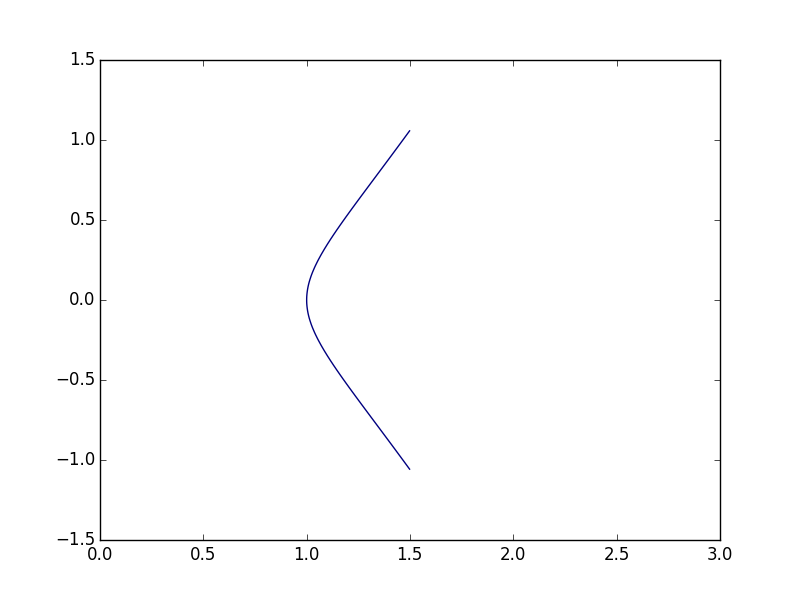
\includegraphics[scale = .75]{3i}

Since both entries of $Dg(x,y) = 0$ at the singular points, we have that \[N_{\mathbf{x}}S = \mathbb{R}^2 \qquad N_{\mathbf{x}}S^{\perp} = \{\mathbf{0}\}\]
\\\\

\subsection*{10.3 (ii)}
\[ Dg(x,y) = \begin{bmatrix}
3x^2 + 2x \\
-2y 
\end{bmatrix}  
= \begin{bmatrix}
0 \\
0 
\end{bmatrix} \]
\[ \implies x = 0, -\frac{2}{3}, y = 0 \]
\[\text{singular points}: (0,0), (-\frac{2}{3}, 0)\]

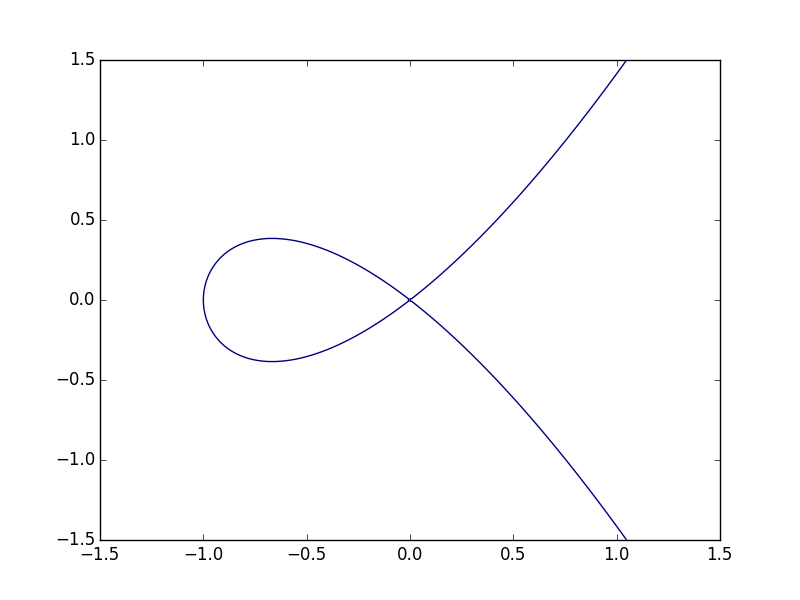
\includegraphics[scale = .75]{3ii}

Since both entries of $Dg(x,y) = 0$ at the singular points, we have that \[N_{\mathbf{x}}S = \mathbb{R}^2 \qquad N_{\mathbf{x}}S^{\perp} = \{\mathbf{0}\}\]
\\\\

\subsection*{10.3 (iii)}
\[ Dg(x,y) = \begin{bmatrix}
3x^2 \\
-2y 
\end{bmatrix}
= \begin{bmatrix}
0 \\
0 
\end{bmatrix} \]
\[ \implies x = 0, y = 0 \]
\[ \implies \text{Singular point}:(0,0)\]

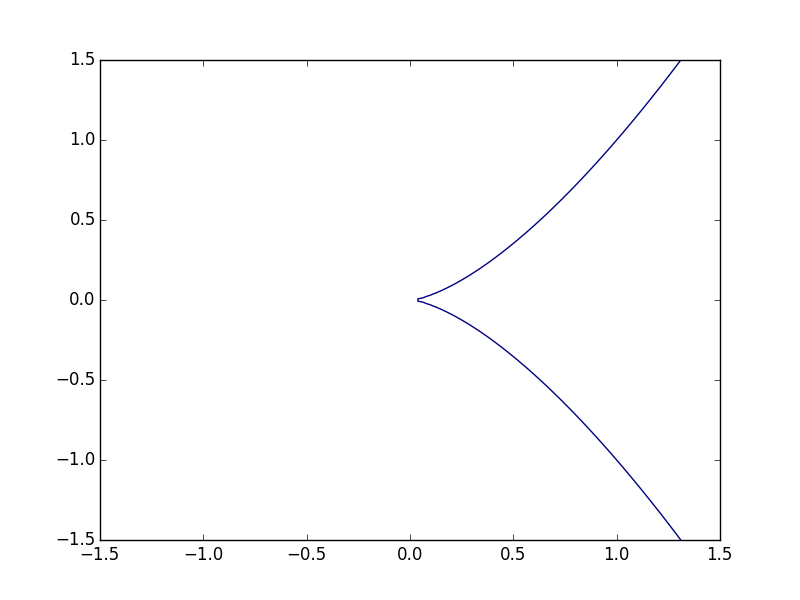
\includegraphics[scale = .75]{3iii}

Since both entries of $Dg(x,y) = 0$ at the singular points, we have that \[N_{\mathbf{x}}S = \mathbb{R}^2 \qquad N_{\mathbf{x}}S^{\perp} = \{\mathbf{0}\}\]
\\\\

\subsection*{10.3 (iv)}
\[ Dg(x,y,z) = \begin{bmatrix}
-2x \\
2y \\
2z 
\end{bmatrix} 
= \begin{bmatrix}
0 \\
0 \\
0 
\end{bmatrix} \]
\[ \implies x=0, y=0, z=0 \]

\[ \implies \text{Singular point}: (0,0,0)\]

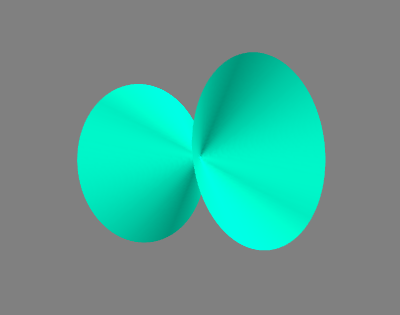
\includegraphics[scale = .75]{3iv}

Since all entries of $Dg(x,y,z) = 0$ at the singular points, we have that \[N_{\mathbf{x}}S = \mathbb{R}^3 \qquad N_{\mathbf{x}}S^{\perp} = \{\mathbf{0}\}\]
\\\\

\subsection*{10.3 (v)}

\[ Dg(x,y,z) = \begin{bmatrix}
2xy \\
x^2 \\
-2z 
\end{bmatrix}
= \begin{bmatrix}
0 \\
0 \\
0 
\end{bmatrix} \]
\[ \implies x = 0, z = 0, y \in \mathbb{R} \]


As $y$ can be any real number, granted that $x=0, z=0$, we have an infinite amount of singular points.

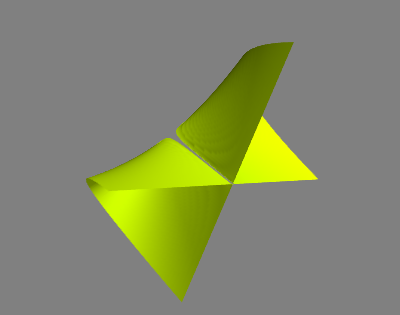
\includegraphics[scale = .75]{3v}

Since all entries of $Dg(x,y,z) = 0$ at the singular points, we have that \[N_{\mathbf{x}}S = \mathbb{R}^3 \qquad N_{\mathbf{x}}S^{\perp} = \{\mathbf{0}\}\]



\subsection*{10.4}


From $3.44 (ii)$, we know that $A^HA$ has the same rank as A. So $Rank(A^HA) = m$ and is invertible so $(A^HA)^H=AA^H$ must likewise be invertible.

\subsection*{10.6}
Lagrange is as follows:
\[\mathscr{L}=x^2+2xy+3y^2+4x+5y+6z+\lambda(3-2y-x)+\mu(6-4x-5z)\]
Our first-order conditions being as follows:
\[\frac{d\mathscr{L}}{dx}=2x+2y+4-\lambda-4\mu=0\]
\[\frac{d\mathscr{L}}{dy}=2x+6y+5-2\lambda=0\]
\[\frac{d\mathscr{L}}{dz}=6-5\mu=0\]
\[\frac{d\mathscr{L}}{d\lambda}=3-2y-x=0\]
\[\frac{d\mathscr{L}}{d\mu}=6-4x-5z=0\]
Which yields the system of equations
\[2x-2y-\frac{33}{5}=0\]
\[3-2y-x=0\]
\[6-4x-5z=0\]
And we get that
\[x=\frac{16}{5}\]
\[y=-\frac{1}{10}\]
\[z=-\frac{34}{25}\]


\subsection*{10.8}

We will attempt to do find the second order conditions using the following equation:
\[D^2\mathscr{L}=
\begin{bmatrix}
D^2f+\mathbf{\lambda}D^2G & DG^T\\
DG & 0 \end{bmatrix}=\begin{bmatrix}
2&2&0&1&4\\
2&6&0&2&0\\
0&0&0&0&5\\
1&2&0&0&0\\
4&0&5&0&0 \end{bmatrix}
\]
The eigenvalues are as follows: \[\lambda_1=-6.14   \qquad \lambda_2=8.19 \qquad\lambda_3=5.85\qquad\lambda_4=0.77\qquad\lambda_5=0.66\] this would indicate neither positive or negative definites conclusively, so the point must be a saddle point. 

\subsection*{10.14}

The volume of a box with consisting of sides with lengths $x,y,z$ can be expressed as $V = xyz$. Therefore, the lagrangian can be written as follows:
\[\mathscr{L}(x,y,z,\lambda) = xyz - \lambda(\frac{x^2}{a^2} + \frac{y^2}{b^2} + \frac{z^2}{c^2} -1)\]
With first-order conditions as follow:
\[\frac{\partial\mathscr{L}}{\partial x} = yz - 2 \frac{\lambda}{a^2}x = 0\]
\[\frac{\partial\mathscr{L}}{\partial y} = xz - 2 \frac{\lambda}{b^2}y = 0\]
\[\frac{\partial\mathscr{L}}{\partial z} = xy - 2 \frac{\lambda}{c^2}z = 0\]
\[\frac{\partial\mathscr{L}}{\partial \lambda} = \frac{x^2}{a^2} + \frac{y^2}{b^2} + \frac{z^2}{c^2} -1 = 0\]
\\We get \[x = \pm \sqrt{\frac{4\lambda^2}{b^2c^2}} \qquad y = \pm \sqrt{\frac{4\lambda^2}{a^2c^2}}, \qquad \pm \sqrt{\frac{4\lambda^2}{a^2b^2}}\]
Plugging this into the constraint we get the following:
\[\lambda = \pm \frac{abc}{\sqrt{12}}\]
Plugging in for $\lambda$, we get \[x^* = \pm \frac{a}{\sqrt{3}}\qquad y^* = \pm \frac{b}{\sqrt{3}} \qquad z^* = \pm \frac{c}{\sqrt3}\] Since $x^*, y^*, z^*$ are half the lengths of the box's sides, we have that the maximum volume is \[8x^*y^*z^* = \frac{8abc}{3\sqrt3}\]


\subsection*{10.17}


We have that
\[\mathscr{L}(x_1,x_2,\lambda) = x_1x_2 + \lambda(x_1+x_2^2-2)\]
Therefore, 
\[\frac{\partial\mathscr{L}}{\partial x_1}=x_2+\lambda=0\]
\[\frac{\partial\mathscr{L}}{\partial x_2}=x_1+2x_2\lambda=0\]
\[\frac{\partial\mathscr{L}}{\partial \lambda}=x_1+x_2^2-2=0\]

 \[ \implies x_{1}^{*} = \frac{4}{3}, \qquad x_2^*=\sqrt{\frac{2}{3}}\]
so we have that $x_2^*$ is the maximum.

\subsection*{10.20}
$\\$The Lagrangian is given as follows:
\[\mathscr{L}=\mathbf{x}^T\mathbf{x}-\lambda(\mathbf{c}^T\mathbf{x}-b)\]
The first-order conditions are as follows:
\[\frac{\partial\mathscr{L}}{\partial\textbf{\textbf{x}}}=2\mathbf{x}-\lambda\mathbf{c}=0\]
\[\frac{\partial\mathscr{L}}{\partial\lambda}=\textbf{c}^T\textbf{x}-b=0\]
And we get the following system of equations:
\[\textbf{x}=\frac{\lambda \mathbf{c}}{2}\]
\[\textbf{c}^T\textbf{x}=b\]
\[\implies \lambda \textbf{c}^T \textbf{c}=2b \]
\[\implies \lambda=\frac{2b}{||c||^2}\]
And finally
\[\implies \textbf{x}=\frac{bc}{||c||^2}\]


Measure Theory (MT) \\\\

\subsection*{MT.1 (i)}


We must show that the three properties of $\sigma$-algebras hold for $(i)-(iii)$.\\
First, that $X \in  \cap _{\alpha \in I} \mathscr{F}_\alpha$. Each $\mathscr{F}_\alpha $ is a $\sigma$-algebra, so it follows that \[X \in \mathscr{F}_\alpha \qquad \forall \alpha\in I\]\[ \implies X \in \cap_{\alpha\in I}\mathscr{F}_\alpha\]

\subsection*{MT.1 (ii)}

Next, that if \[A \in \cap_{\alpha\in I}\mathscr{F}_\alpha \implies A^{C} \in\cap_{\alpha\in I}\mathscr{F}_\alpha\] As \[A \in \cap_{\alpha\in I}\mathscr{F}_\alpha \implies \forall \alpha \in I, A \in \mathscr{F}_\alpha\]. But we know that $\mathscr{F}_\alpha$ is a $\sigma$-algebra, so we have that \[A^C \in \mathscr{F}_\alpha \qquad \alpha\in I \implies A^C \cap_{\alpha\in I}\mathscr{F}_\alpha\] \\

\subsection*{MT.1 (iii)}

Next, if we have a set $\{A_i\}$ such that \[\{A_i\}_{i=1}^{\infty} \subset \cap_{\alpha\in I}\mathscr{F}_\alpha \implies \cup_{i=1}^{\infty}A_i \in \cap_{\alpha\in I}\mathscr{F}_\alpha\]
Note that
\[\{A_i\}_{i=1}^{\infty} \subset \cap_{\alpha\in I}\mathscr{F}_\alpha \implies \{A_i\}_{i=1}^{\infty} \subset \mathscr{F}_\alpha \qquad \alpha \in I\]
Also, as each $\mathscr{F}_\alpha$ is a $\sigma$-algebra, we have that
\[\cup_{i=1}^{\infty}A_i \in \mathscr{F}_\alpha \quad \alpha \in I\]\[ \implies \cup_{i=1}^{\infty}A_i \subset \cap_{\alpha\in I}\mathscr{F}_\alpha\]\\
With all these facts, we have that $\cap_{\alpha\in I}\mathscr{F}_\alpha$ is a  $\sigma$-algebra.\\\\




\subsection*{MT.2 (i)}

As $\mathscr{B}$ is the Borel $\sigma$-algebra of $\mathbb{R}$, we have that \[\mathscr{B} = \{(a,b) | a<b, \forall a,b\in \mathbb{R}\}\] We need to show that all intervals of the forms $(-\infty,x)$, $(-\infty,x]$, $(x,y]$, and $[x,y]$, as well as the singleton set $\{x\}$, are all in $\mathscr{B}$. \\
Let us express $(-\infty, x)$ as \[\cup_{i=1}^{\infty}(x-i, x)\]Note that this is the countable union of open intervals. \[ \implies (-\infty, x) \in \mathscr{B}\] \\


\subsection*{MT.2 (ii)}

Let us express $(-\infty, x]$ as follows: \[ (x, \infty)^C = (\ \cup_{i=1}^{\infty}(x, x+i)\ )^C \] This is the complement of the countable union of open intervals, which are in $\mathscr{B}$. \[ \implies (-\infty, x] \in \mathscr{B}\] \\

\subsection*{MT.2 (iii)}

Let us express $(x,y]$ as follows: \[ (\ (-\infty, x] \cup (y, \infty)\ )^C \]

By $(i),(ii)$, we have that 
\begin{align*}
(-\infty,x] \in \mathscr{B} \text{and} (y, \infty)^{C} \in \mathscr{B} &\implies (y, \infty) \in \mathscr{B}
\\&\implies (\ (-\infty, x] \cup (y, \infty)\ ) \in \mathscr{B} \\&\implies (\ (-\infty, x] \cup (y, \infty)\ )^C=(x,y] \in \mathscr{B}
\end{align*} 

\subsection*{MT.2 (iv)}

Let us express $[x,y]$ as follows:
\[ (\ (-\infty, x) \cup (y, \infty)\ )^C\]By parts $(i)-(iii)$, we see that \[(\ (-\infty, x) \cup (y, \infty)\ )^C \in \mathscr{B} \implies [x,y] \in \mathscr{B}\]

\subsection*{MT.2 (v)}

Let us express $\{x\}$  as follows: \[(\ (-\infty, x) \cup (x, \infty)\ )^C \in \mathscr{B}\]\\\\


\subsection*{MT.3}

Let us first re-index the $\alpha_i$'s so that they are monotonically increasing. Then we have the following: \[x \in A_i, s(x) = \alpha_i \geq \alpha_{i-1} \geq \hdots \geq \alpha_1\] We can show with this fact that $s^{-1}((-\infty,a))$ is measurable where $a \in \mathbb{R}$. \\
As the sum approaches some finite $n$, the range of $A$ is finite. Moreover, because we have re-indexed the $\alpha_i$'s, granted that$a \in A_1$ \[ \implies s^{-1}((-\infty,a)) = A_1\] Granted that $a \in A_2$ \[ \implies s^{-1}((-\infty,a))=A_1 \bigcup A_2 \] Continuing inductively, we get, for large values of $a$ that \[s^{-1}((-\infty,a))=A_1 \bigcup A_2 \hdots \bigcup A_n \] This implies that at worst, $s^{-1}((-\infty,a))$ is the union of $n$ measurable sets, which is measurable. $s$, therefore, must be measurable.

\subsection*{MT.4}

We want to show that
\[v(\cup_{i=1}^\infty A_i) = \sum_{i=1}^\infty v(A_i)\]
Note that
\begin{align*}
\implies v(\cup_{i=1}^\infty A_i)&=\mu((\cup_{i=1}^\infty A_i) \cap D)\\
&=\mu(\cup_{i=1}^\infty (A_i \cap D))
\end{align*}
by DeMorgan's Laws.
Since $D \in F$ we have that \[A \cap D \in F \quad  \forall A \in F\] As $\mu$ is a measure on $F$ we have
\[\mu(\cup_{i=1}^\infty (A_i \cap D))=\sum_{i=1}^\infty \mu(A_i \cap D)=\sum_{i=1}^\infty v(A_i \cap D)\]
\[ \implies v(\cup_{i=1}^\infty A_i) = \sum_{i=1}^\infty v(A_i) \]  $\implies v$ is a measure on $F$. \\\\

\subsection*{MT.4}

Note that \[f(x)=x^2+1 \quad  \forall x \in \Omega = \{-5,-4,-3,-2,-1,0,1,2,3,4,5 \}\] In order to express $f$ as a simple function, let $\alpha_i \in \alpha$ be expressed as follows:
\[\alpha=\{26,17,10,5,2,1,2,5,10,17,26\}\]
So $f: \Omega \rightarrow \mathbb{R}$ can be expressed as a simple function $s$ according to the following:
\[s(x)=\sum_{i=1}^{11}\alpha_i \chi_{A_i}(x)\]
Where  \[A_1=\{-5\}, A_2=\{-4\}, \hdots A_{10}=\{4\}, A_{11}=\{5\}\]
Now, $f$ is simple and therefore measurable by MT.3. 
\[\implies \int_\Omega f d\mu=\sum_{i=1}^{11}\alpha_i\mu(A_i \cap \Omega )\] 
Our measure is given by $\mu (\{x\}) = \frac{1}{|x|}$ where $x \neq 0$, and $\mu (\{x\}) = 0$ where $ x = 0$. 
And since $A_i \cap \Omega = A_i$ 
\[\implies  \int_\Omega f d\mu=\sum_{i=1}^{11}\alpha_i\mu(A_i ) \] \[=
26(\frac{1}{5}) + 17(\frac{1}{4}) + 10(\frac{1}{3}) + 5(\frac{1}{2}) + 2(1) + 1(0) + 2(1) + 5(\frac{1}{2}) + 10(\frac{1}{3})+ 17(\frac{1}{4}) +26(\frac{1}{5})\]
\[=1037/30 \approx 34.566\]



\end{document}
 






